\documentclass[12pt]{article}

\pagestyle{empty}

\newcommand{\spifff}{\qquad\text{iff}\qquad}
\newcommand{\spand}{\qquad\text{ and }\qquad}
\newcommand{\forward}{\noindent ($\Longrightarrow$) \,\,}
\newcommand{\back}{\noindent ($\Longleftarrow$) \,\,}
\newcommand{\R}{\mathbb R} %REALS
\newcommand{\C}{\mathbb C} %COMPLEX
\newcommand{\N}{\mathbb N} %NATURAL NUMBERS
\newcommand{\Q}{\mathbb Q} %RATIONALS
\newcommand{\Z}{\mathbb Z} %INTEGERS

\usepackage{amsmath}
%\usepackage{amsthm}
\usepackage{graphicx}  
\usepackage{amssymb}   
\usepackage{enumerate}

\newcommand{\comp}[1]{#1^{\cal C}}
\newcommand{\ray}[1]{\overrightarrow{#1}}
\renewcommand{\line}[1]{\stackrel{\longleftrightarrow}{#1}}
\renewcommand{\deg}{^{\circ}}
\newcommand{\seg}[1]{\overline{#1}}

\newenvironment{solution}{\noindent {\bf Solution:}}{\hfill \rule{1mm}{3mm} \bigskip}
\newenvironment{proof}{\noindent {\bf Proof:}}{\hfill
\rule{1mm}{3mm} \bigskip}

\usepackage{amsmath}
%\usepackage{amsthm}
\usepackage{graphicx}  
\usepackage{amssymb}   
\usepackage{enumerate}

\begin{document}
\begin{center}
{\bf Takehome Midterm}\\
Sam Chong Tay\\
Euclidean and Non-Euclidean Geometry\\
Fall, 2012
\end{center}

\begin{enumerate}

\item {\em Undefined terms {\bf abba} and {\bf dabba}.}

\begin{description}
	\item[{\bf Axiom I.}] There exist at least two dabbas.
	\item[{\bf Axiom II.}] Every abba is a set of at least two dabbas.
	\item[{\bf Axiom III.}] If $c$ and $d$ are distinct dabbas, then there exists one and only one abba that contains both $c$ and $d$. 
	\item[{\bf Axiom IV.}] If $a$ is an abba, then there exists a dabba $d$ that is not in $a$.  
	\item[{\bf Axiom V.}] If $a$ is an abba, and $d$ is a dabba not in $a$, then there exists one and only one abba containing $d$ and not containing any dabba that is in $a$.  
\end{description}


\begin{enumerate}
	\item (2 pts.) Prove that every dabba is contained in at least two abbas.
	
	\begin{proof} Let $d$ be a dabba. We wish to show that there exist two abbas $A$ and $B$ such that $d\in A$ and $d\in B$. By Axiom I there exists a dabba $c\ne d$. By Axiom III there exists a unique abba $A$ such that $c, d \in A$. By Axiom IV there exists a dabba $e\notin A$. Hence $d\ne e$ so again by Axiom III there exists a unique abba $B$ such that $d, e \in B$. Of course since $e\notin A$ and $e\in B$, we know that $A\ne B$. Therefore the dabba $d$ is contained in two distinct abbas $A$ and $B$.
	\end{proof}
	
	\item (3 pts.) Prove that there exist at least four distinct dabbas.
	
		\begin{proof} We know there exist two distinct dabbas $c$ and $d$ from Axiom I. By Axiom III there exists a unique abba $A$ such that $c,d\in A$. By Axiom IV there exists a dabba $e\notin A$. Now by Axiom 5 there exists a unique abba $B$ containing $e$ and not containing any dabba that is in $A$, so that $c\notin B$ and $d\notin B$. But by Axiom II there must exist another dabba $f\in B$, where $f\ne e$. All that is left is to justify that $c,d,e,$ and $f$ are all distinct. We know that $c\ne d$ and $e\ne f$ by construction of the abbas $A$ and $B$ respectively. Since $c,d \notin B$, we also have $c\ne e, c\ne f, d\ne e, $ and $d\ne f$. Therefore these are four distinct dabbas.
	\end{proof}
	
	\item (2 pts.) Are the real numbers, together with the set of subsets of the real numbers a model for the abba/dabba system?  Why or why not?
	
		\begin{solution} No! Of course the only reasonable interpretation in this scenario would be to have $\R$ as the set of dabbas and $\cal{P}(\R)$ as the set of abbas, since each abba contains two dabbas and certainly a real number $r$ does not contain two subsets of $\R$, as $r$ is not a set. So considering  $\R$ as the set of dabbas and $\cal{P}(\R)$ as the set of abbas, there are many reasons this model does not work. Perhaps the most immediate reason is the failure to satisfy Axiom II, as the empty set and any singleton is a subset of $\R$ that does not contain two real numbers. (In fact, this model cannot satisfy any of the axioms II-V.)
	
	\end{solution}
	
	\item (3 pts.) Construct a finite model of the the abba/dabba system. 
		
		\begin{solution} The figure below depicts a model of the abba/dabba system, where the dabbas are $w,x,y,z$ and the abbas are $$A=\{x,w\},\quad B=\{w,y\},\quad C=\{x,z\},$$ $$ D=\{w,z\},\quad E=\{x,y\},\quad F=\{y,z\}.$$
		
	\begin{center}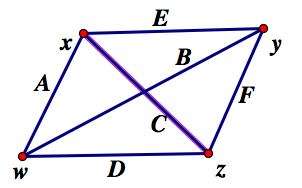
\includegraphics[width=2.7in]{abbdabba.png}\end{center}
	\end{solution}
	
	
\end{enumerate}

\item Let $A$, $B$, $C$ and $D$ be points.  Suppose that $A \ast B \ast C$ and $A \ast C \ast D$. 

\begin{enumerate}
	\item (5 pts.) Prove that $\line{AB} \ =\  \line{CD}$.  
	
		\begin{proof} By definition of betweenness, the points $A,B,C$ are distinct and collinear, and the points $A,C,D$ are distinct and collinear. So let $\ell$ and $m$ be the lines such that
		$$A,B,C\in\ell \spand A,C,D\in m.$$ Note here that since $A,B$ are distinct and $C,D$ are distinct, we have $\ell =\ \line{AB}$ and $m=\ \line{CD}.$ By the Incidence Postulate, since $A$ and $C$ are distinct, there is exactly one line containing both $A$ and $C$. Therefore we must have $\ell = m$, so that $\line{AB} \ =\  \line{CD}$.  
	\end{proof}
	
	\item (10 pts.) Prove that $B \ast C \ast D$ and $A \ast B \ast D$.  
	
		\begin{proof} Recall from part (a) that $A,B,C,$ and $D$ all lie on one line, which we will call $\ell$. Since $A$ and $C$ are distinct, by the Ruler Placement Postulate we can construct a coordinate function $f:\ell \to \R$ such that $f(A)=0$ and $f(C)>0$. Since $A*B*C$, the Betweenness Theorem for Points guarantees that either $f(A) < f(B) < f(C)$ or $f(C)<f(B)<f(A).$ Of course in our construction we have $f(A) < f(C),$ so we must have $$f(A) < f(B) < f(C).$$ Similarly, since $f(A)<f(C)$ and $A*C*D$, the Betweenness Theorem for Points implies that $f(A) < f(C) < f(D).$ Then of course altogether we have $$f(A)<f(B)<f(C)<f(D),$$ and again the same theorem guarantees that $$B*C*D \spand A*B*D.$$\end{proof}
\end{enumerate}

\item (10 pts.) Given an angle $\angle CAB$ where $A,B,C$ are noncollinear and $D \in \ \line{BC}$, prove that $D$ lies in the interior of $\angle CAB$ if and only if $B \ast D \ast C$.  

	\begin{proof} As above, let $A,B,$ and $C$ be noncollinear and $D \in \ \line{BC}$. By Theorem 3.3.10\footnote{This was proved in class by Ben Tanoff.} we know that $B*D*C$ if and only if the ray $\ray{AD}$ is between the rays $\ray{AC}$ and $\ray{AB}$. But by Definition 3.3.8, we know that the ray $\ray{AD}$ is between the rays $\ray{AC}$ and $\ray{AB}$ if and only if $D$ is in the interior of $\angle CAB$.	Therefore we conclude that $D$ lies in the interior of $\angle CAB$ if and only if $B \ast D \ast C$. \end{proof} %Since $A,B,C$ are noncollinear, we can consider the triangle $\triangle ABC$.
	
	%\forward Suppose that $D$ is in the interior of $\angle CAB$. By Definition 3.3.8 this means that $\ray{AD}$ is between rays $\ray{AC}$ and $\ray{AB}$.
	 %Then we know by the Crossbar Theorem that there exists a point $G$ such that $G$ lies on both $\ray{AD}$ and $\seg{BC}$. Also we have $\line {AD} \ne \line{BC}$, as this would contradict the noncollinearity of $A,B,$ and $C$. Therefore by Problem 3.2.1, $G$ is the only point in the intersection  $\line{AD} \cap \line{BC}$. However we are assuming $D\in\line{BC}$ and clearly $D\in\line{AD}$. Therefore we must have $G=D$, and from above this means that $D\in\seg{BC}$.
	

	
\item (10 pts.) Suppose $A$, $B$ and $M$ are collinear and $A\ne B$.  Prove that $M$ is the midpoint of $\seg{AB}$ if and only if $MA = MB$. 

	\begin{proof} \forward The forward direction is trivial; if $M$ is the midpoint of $\seg{AB}$, then by definition $MA=MB$.
	
	\back Suppose $MA=MB$. To conclude that $M$ is the midpoint of $\seg{AB}$, we need only show that $A*M*B$. Since $A,B,$ and $M$ are collinear, we can consider the exhaustive cases \begin{enumerate}[(i)] \item{ $M*A*B$ \ or \ $A*B*M$,} 
	\item{$M=A$ \ or \ $M=B$, \ or}
	\item{$A*M*B$.}
\end{enumerate}
In case (i) we can assume without loss of generality that $M*A*B$. Then $MB = MA + AB,$ but we know $AB>0$ since $A$ and $B$ are distinct. This would imply that $MB \ne MA$, contradicting our hypothesis. In case (ii) we can suppose without loss of generality that $M=A$. Then $$0=MA=MB=AB,$$ which contradicts $A\ne B$. Therefore the only other possibility is that $A*M*B$, and we conclude that $M$ is the midpoint of $\seg{AB}$.
	\end{proof}

\item (10 pts.) Prove the {\em Hypotenuse and Acute-angle Congruence Condition}:  If the hypotenuse and an acute angle of one right triangle are congruent to the hypotenuse and an acute angle of another right triangle, then the triangles are congruent.

	\begin{proof} Let $\triangle ABC$ and $\triangle DEF$ be right triangles with right angles at the vertices $C$ and $F$ respectively. Suppose further that $\seg{AB}=\seg{DE}$ and $\angle BAC \cong \angle EDF$.
	\begin{center}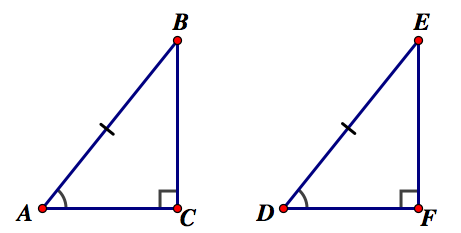
\includegraphics[width=3in]{5_1.png}\end{center}
Let $C'\in \ray{AC}$ such that $AC'=DF$. Then we have $\seg{AB}\cong\seg{DE}$, $\angle BAC'=\angle BAC\cong\angle EDF,$ and $\seg{AC'}\cong\seg{DF}$, so by SAS we conclude that \begin{equation}\label{1} \triangle ABC' \cong \triangle DEF \end{equation}
We wish to show that $C'=C,$ which will prove the claim. Since $C'\in\ray{AC}$ there are just a few other cases to rule out: (i) $C'=A$, (ii) $A*C'*C$, and (iii) $A*C*C'$.

\noindent(i) First if $A=C'$ then $0=AC'=DF$, implying $D=F$. But then $D,E,F$ would not be collinear and $\triangle DEF$ would not exist! This obviously contradicts the hypothesis.

\noindent(ii) If $A*C'*C,$ it follows that $B,C,C'$ are noncollinear; we know that $A,B,C$ are noncollinear, so that $B \notin \line{AC}$. But in this case, $\line{AC}=\line{C'C}$, which implies that $B,C,C'$ are noncollinear and thus we can consider triangle $\triangle BCC'$.
\begin{center}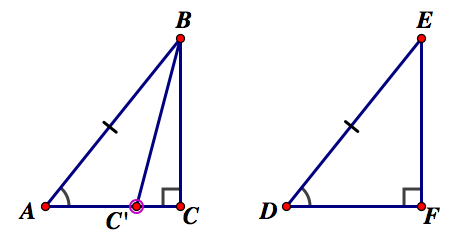
\includegraphics[width=3in]{5_2.png}\end{center}
In this case we have $\angle BC'\!A$ as an exterior angle to triangle $\triangle BCC'$, with a remote interior angle $\angle BCC'$. But by the constructed triangle congruence in (\ref{1}), we have $\mu(\angle BC'\!A) = \mu(\angle EFD)=90\deg$. However in this case $\angle BCC'= \angle BCA$ which we also defined as a right angle. This contradicts the Exterior Angle Theorem.

\noindent(iii) If $A*C*C'$, then for the same reasons given in case (ii), we have $B,C,C'$ noncollinear so that we can consider triangle $\triangle BCC'$.
\begin{center}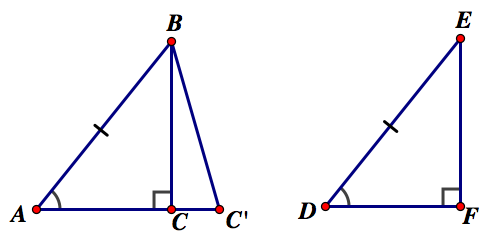
\includegraphics[width=3in]{5_3.png}\end{center}
First note that $\angle BCA$ is an exterior angle to $\triangle BCC'$ with remote interior angle $\angle BC'C$. Also in this case, $\angle BC'\!C = \angle BC'\!A$. Thus by congruence (1) we have
$$ \mu(\angle BC'C) = \mu(\angle BC'\!A)= \mu (\angle EFD) = 90\deg.$$ However we defined $\angle BCA$ as a right angle, and this contradicts the Exterior Angle Theorem.

Therefore the only other possibility is that $C'=C$, which allows us to conclude that $\triangle ABC=\triangle ABC'$, and thus by congruence (1), $$\triangle ABC \cong \triangle DEF.$$
\end{proof}

\item (5 pts.) Fix points $A$ and $B$ and let $K = \{ P | PA = PB\}$.  One and only one of the following is true.  Which one and why?

\begin{itemize}
		\item $K$ is a singleton set (contains only one point).
		\item $K$ is a ray
		\item $K$ is a segment
		\item $K$ is a triangle
		\item $K$ is the interior of a triangle.
		\item $K$ is a line.
\end{itemize}

	\begin{solution} From the definitions above, we have two scenarios. If $A=B$, then the set $K$ is easily seen to be every point in the plane. I believe the case that you are looking for in this question is when $A\ne B$. With $A$ and $B$ distinct we see from the Pointwise Characterization of Perpendicular Bisectors that $K$ is precisely the perpendicular bisector of segment $\seg{AB}$. Thus, the answer is that $K$ is a line. \end{solution}

\item (10 pts.) Let $A$, $B$, and $C$ be non-collinear points;  This question concerns the triangle $\triangle ABC$.  Let $M$, $P$ and $Q$ be the midpoints of the sides $\seg{AB}$, $\seg{AC}$ and $\seg{BC}$.  Suppose that the perpendicular bisectors $\ell$ and $m$ of sides $\seg{AB}$ and $\seg{AC}$ intersect at point $R$, all as shown in the diagram.  Show that the perpendicular bisector $n$ of $\seg{BC}$ also goes through the point $R$. (This point is called the {\em circumcenter} of the triangle.)

\begin{center}
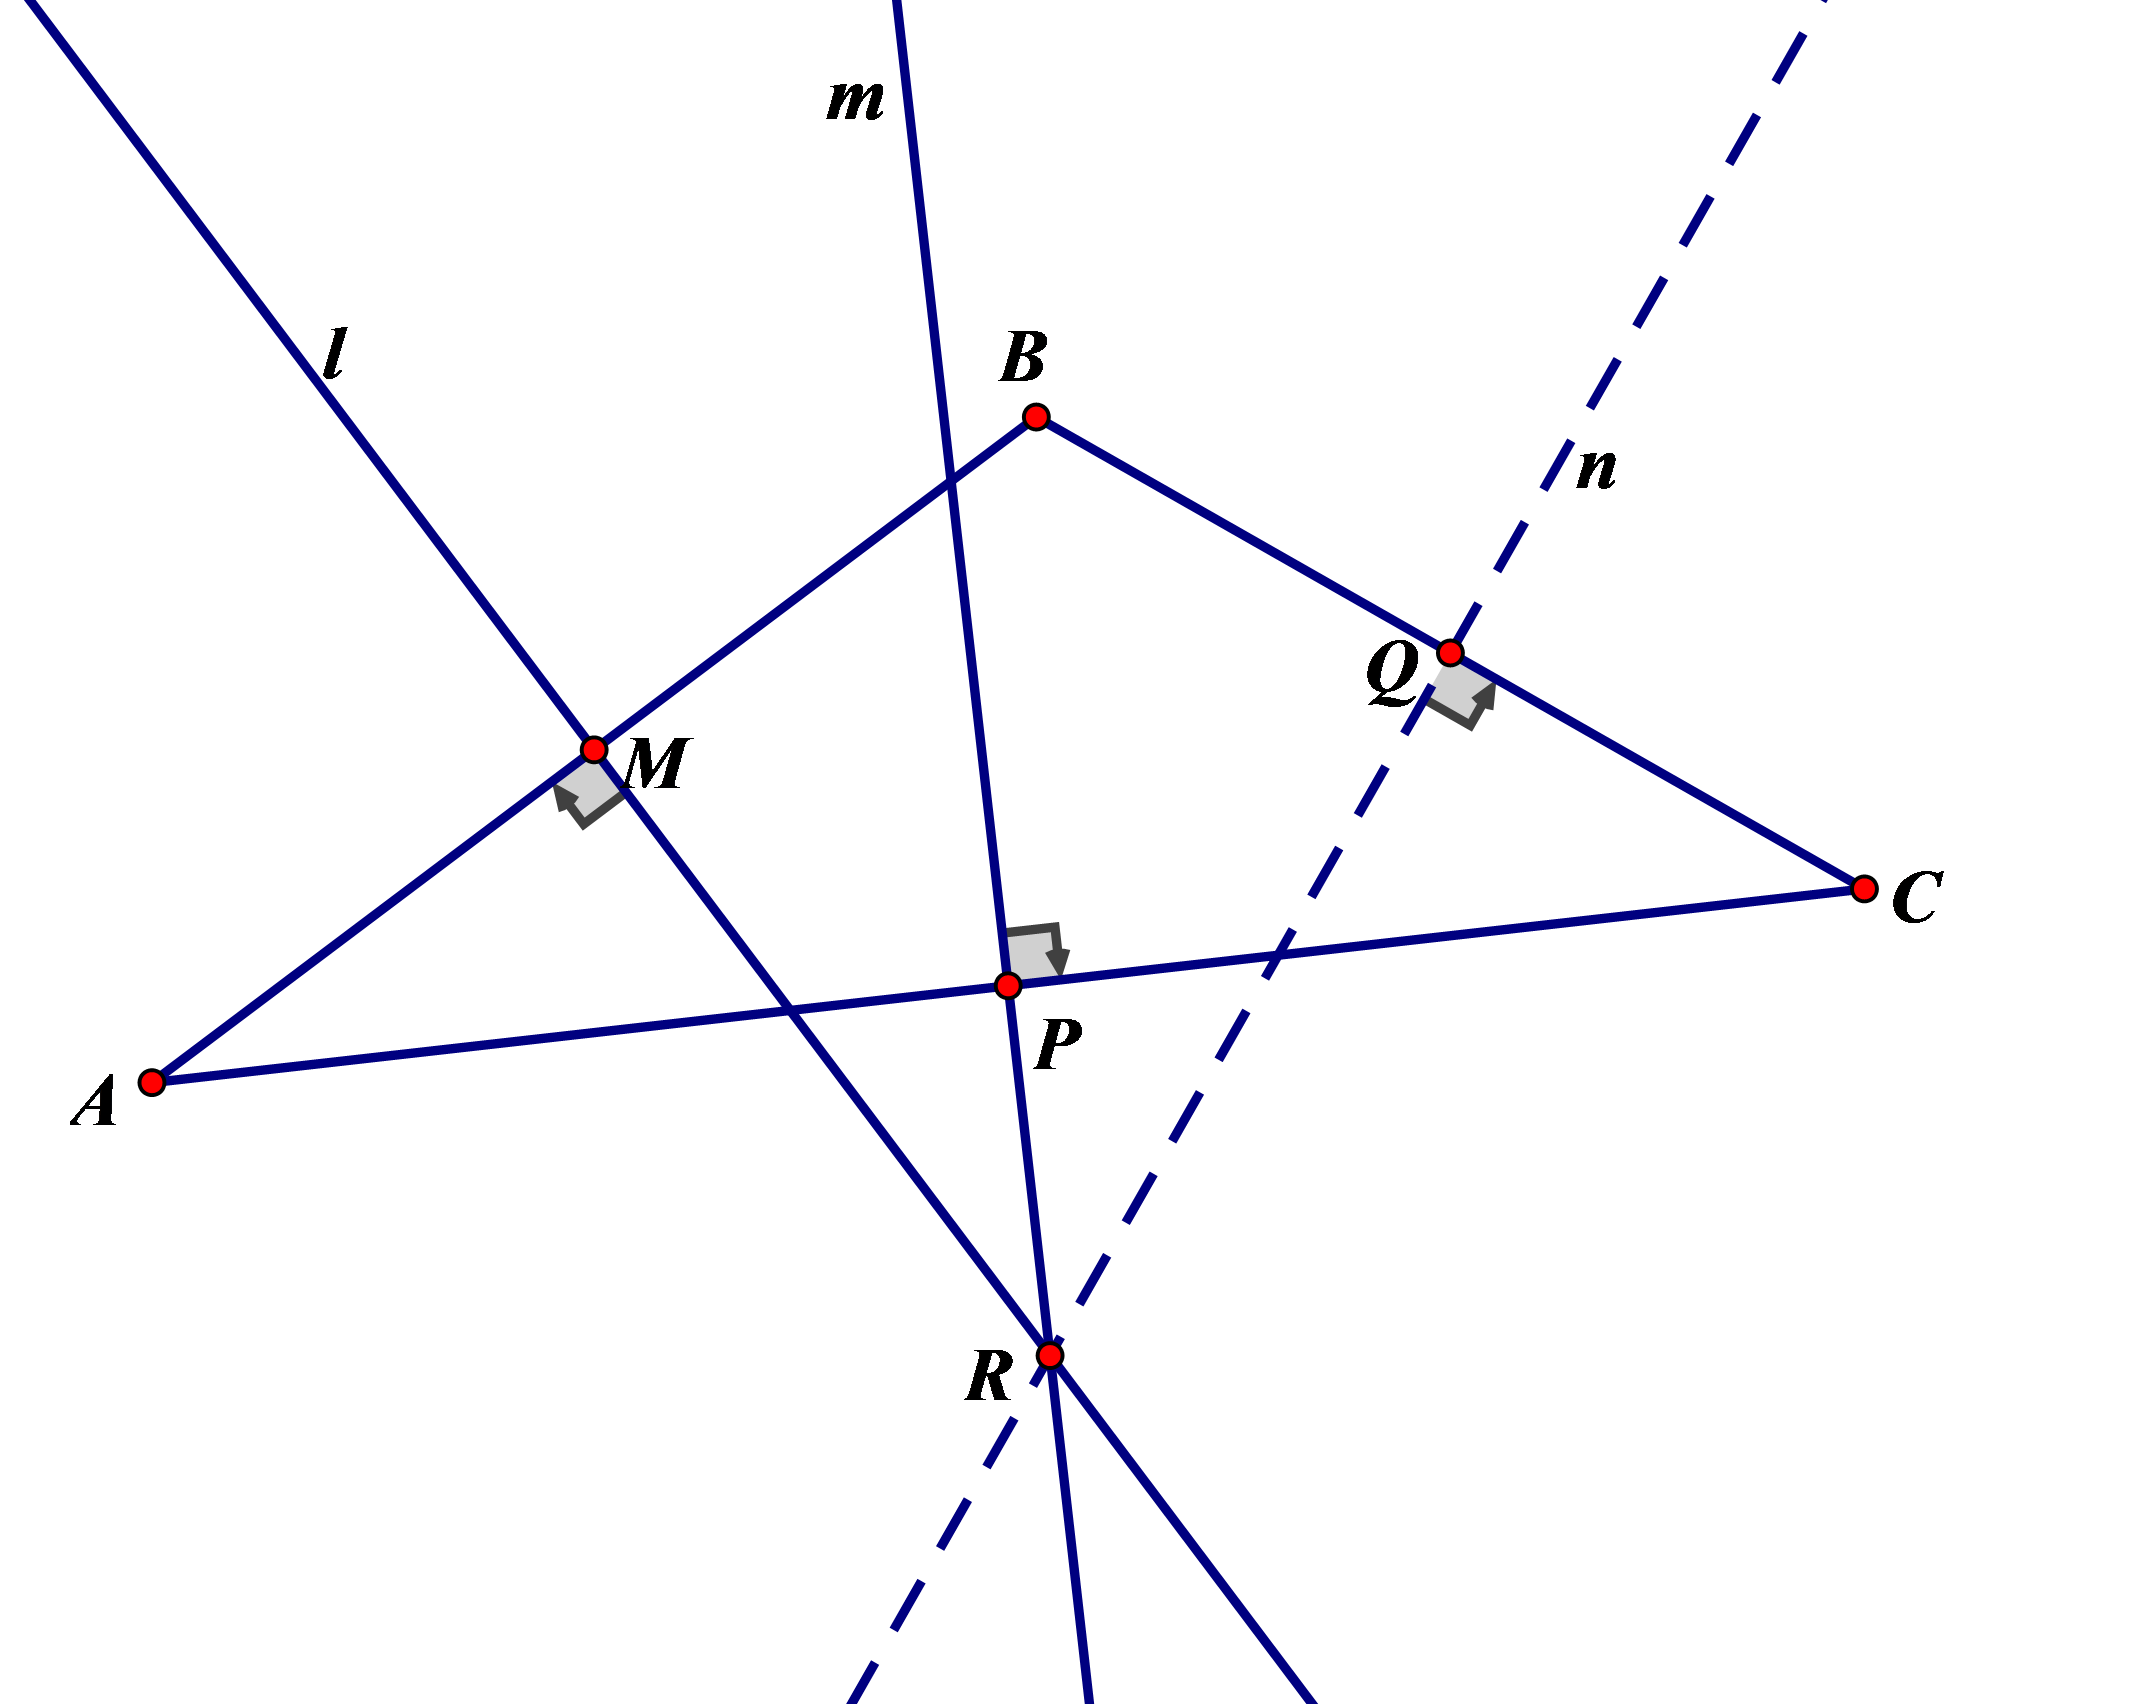
\includegraphics[height=2.5in]{midtermF12_1.png}
\end{center}

	\begin{proof} Let  $A$, $B$, and $C$ be non-collinear (and thus distinct) points and consider the triangle $\triangle ABC$. Let $\ell, m$ and $n$ be the perpendicular bisectors of segments $\seg{AB}, \seg{AC},$ and $\seg{BC}$ respectively. Suppose that $\ell$ and $m$ intersect at a point $R$. By the Pointwise Characterization of Perpendicular Bisectors we have that since $R\in\ell$ and $R\in m$, $$RA=RB \spand RA=RC.$$ Hence $RB=RC$, and again by the P.C.o.P.B we have $R\in n$, completing the proof.
	\end{proof}
	
\end{enumerate}

\begin{description}
	\item[Bonus] For 1 bonus point, the theorem in Problem~7, captures the familiar geometric principle that 
	\begin{quote}
	Three points determine a \underline{circle!}, as seen below.
	\end{quote}
\begin{center}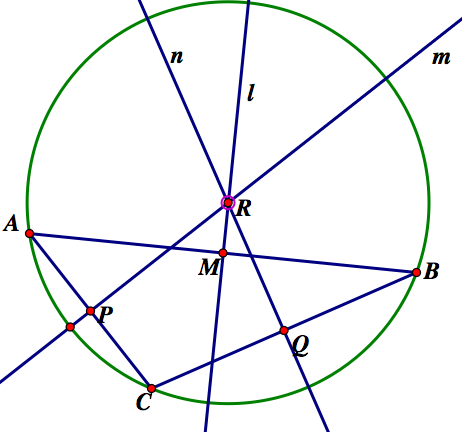
\includegraphics[width=2.5in]{last.png}\end{center}
The circumcenter is the center of the circle and each vertex of the triangle lies on the circumference.
\end{description}
\end{document}